\documentclass[a4paper,10pt,oneside,twocolumn,notitlepage,final,dvipdfmx]{jarticle}
%====================================================================%
\usepackage{ss24_UTF8}
%====================================================================%

%====================================================================%
\usepackage{amsmath, amssymb}
\usepackage{siunitx}
\usepackage{physics}
\usepackage{empheq}
\usepackage[dvipdfmx]{graphicx}
\usepackage{hyperref}
\usepackage{pxjahyper}
\AtBeginDocument{\RenewCommandCopy\qty\SI}
%====================================================================%
\newcommand{\masssolar}{M_\odot}
%====================================================================%
\author{熊田 遼太 (東北大学 天文学専攻 M1)}
\title{原始惑星系円盤における磁気拡散\\とくに両極性拡散が磁気回転不安定性へ与える影響}
%====================================================================%
\begin{document}
%====================================================================%
 \abst{
原始惑星系円盤(円盤)は惑星形成の舞台であり, その効率は円盤内の乱流強度によって決定される. 乱流の生成源は磁気回転不安定性(MRI)と考えられているため, MRIの成長を理解することは惑星形成過程を理解する上で重要となる. 一方, MRIの成長は, 電磁流体の磁気拡散項:オーム散逸, ホール効果, 両極性拡散によって抑制されると考えられている. したがって, これらの効果が円盤へ与える影響を理解することは重要である. しかし,  磁気拡散項がどのくらいMRIを抑制するのかは, オーム散逸を除き十分に理解されていない. 本講演では, オーム散逸と両極性拡散を考慮したshearing--box シミュレーションを初めて行い, MRIの成長を調べたBai \& Stone (2013)\cite{baiWinddrivenAccretionProtoplanetary2013a}をレビューする. シミュレーションは(1)オーム散逸のみ, (2)オーム散逸と両極性拡散 の効果を考慮した場合でそれぞれ実施した. 
シミュレーションの結果, 磁気拡散とくに両極性拡散はMRIの効果を大きく抑制した. 一方で, 磁気遠心力風が角運動量の輸送に大きく貢献していることが分かった. 得られた結果は, MRI由来の乱流粘性により角運動量が輸送されるという, 原始惑星系円盤の従来の描像を変える可能性がある.
}
%=====================================================================%
\section{Introduction}
原始惑星系円盤とは, 原始星周囲に構成される円盤状の構造である. 惑星形成は円盤内で起きると考えられており, それゆえ円盤ガスの降着率$\dot{M}$は惑星形成を考える上で重要となる. 降着率の観測値は\( \dot{M}_\mathrm{obs} \approx 10^{-8\pm 1}\masssolar ~\si{yr^{-1}} \)であることが分かっている\cite{gullbringDiskAccretionRates1998}が, 降着においてどのようなメカニズムが角運動量を輸送しているのかははっきりとしていない. 
\par
角運動量輸送メカニズムの候補のひとつは円盤内で生じた乱流粘性である. この乱流粘性の効果をパラメータとして置き, 計算を行うのが標準円盤モデルである\cite{shakuraBlackHolesBinary1973}. パラメータ$\alpha$は以下で与えられる:
\begin{equation}\label{eq:alphaparametor}
  \alpha c_s^2\Sigma = \int T_{R\phi} \dd{z}
\end{equation}
ここで, $T_{R\phi}$は応力テンソルの$R\phi$成分である:
\begin{equation}
  T_{R\phi} = T_{R\phi}^{\mathrm{Rey}} + T_{R\phi}^{\mathrm{Max}} = \rho v_R v_\phi - B_R B_\phi
\end{equation}
降着率$\dot{M}$は, $\alpha$を用いて以下で与えられる:
\begin{equation}\label{eq:accretionrate}
  \dot{M} = \frac{2\pi}{\Omega}\alpha c_s^2 \Sigma
\end{equation}
ただし$c_s ,\,\Omega ,\,\Sigma$はそれぞれ音速, 円盤の回転角速度, 円盤の面密度である. また, \(T_{R\phi}^{\mathrm{Rey}},\,T_{R\phi}^{\mathrm{Max}},\, \rho \)はReinodls応力の$R\phi$成分, Maxwell応力の$R\phi$成分, 円盤の体積密度であり, $v_R,\,v_\phi,\,B_R,\,R_\phi$はそれぞれ速度, 磁場の$R$成分, $\phi$成分である. のちに説明する磁気回転不安定性が発達している場合には, \(T_{R\phi}^{\mathrm{Max}}\gg T_{R\phi}^{\mathrm{Rey}}\)となる.
\par
一般に円盤内のガスは電離しているため, その流体運動は電磁流体力学(\textbf{m}agneto \textbf{h}ydro\textbf{d}ynamics, \textbf{MHD})で記述される. MHDでは, 運動は主として磁場が駆動する. 磁場の時間変化を与える方程式が, 誘導方程式である:
\begin{empheq}{align}\label{eq:induction_eq}
\begin{split}
    \pdv{\vb{B}}{t} &= \curl(\vb{u}\times\vb{B})\\
  -&\curl[\eta_O\vb{J}+\eta_A\vb{J}_\perp + \eta_H(\vb{J}\times\vb{B})]
\end{split}
\end{empheq}
ここで$\vb{u}$は速度ベクトル, \( \vb{J} \)は電流密度ベクトルであり, 添字$\perp$は磁場$\vb{B}$に対して直交する成分を表す. 右辺第2項が無視できる場合, プラズマは磁力線とともに運動する(凍結定理). この性質が, 後述の磁気回転不安定性を駆動する要因のひとつになる. 
\par
磁気回転不安定性(\textbf{m}agneto\textbf{r}otational \textbf{i}nstability, \textbf{MRI})は, 円盤ガスの差動回転によって生じる流体力学的不安定性である. MRIの成長過程を表した模式図を\figref{fig:MRI}に示した. プラズマは磁力線とともに運動するため, 磁場にゆらぎが生じると, プラズマに差動回転が生じる(図左). 差動回転しているプラズマに対しては磁気張力トルクがはたらき, 内側へ落ち込んだプラズマはより内側へと, 外側へ飛ばされたプラズマはより外側へと, 移動していく(図中央). この移動によって, 磁力線はさらに歪み, 角運動量がより効率的に交換され, 円盤内は乱流状態となる(図右). MRIが角運動量輸送のメカニズムとしてはたらくことはBalbus \& Hawley(1991) が提唱し, 定常円盤降着を考える際の標準モデルとなっている\cite{balbusPowerfulLocalShear1991}. 
\begin{figure}
  \centering
  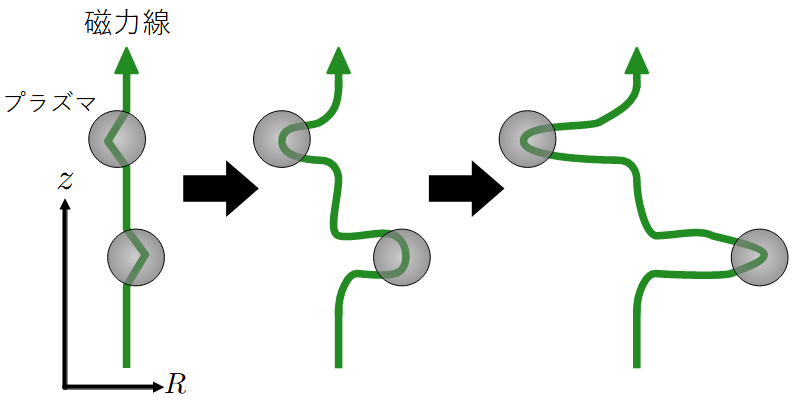
\includegraphics[width=0.9\linewidth]{./contents/MRI.png}
  \caption{磁気回転不安定性(MRI)の模式図. 磁力線のゆらぎ(図左)がプラズマの角運動量を輸送し(図中央), さらに磁力線を歪ませる(図右). }\label{fig:MRI}
 \end{figure}
\par
一方で, 式\eqref{eq:induction_eq}右辺第2項に示された磁場の拡散(磁気拡散)はMRIを抑制する. 磁気拡散の各項はそれぞれ(1)オーム散逸, (2)両極性拡散 (3)ホール効果, と呼ばれている. このうち(3)は, 今回のシミュレーションでは考慮されていないため, 説明を省略する. (1)のオーム散逸は流体の担い手(中性粒子)と電流の担い手(電子)との衝突により生じる磁場の拡散である. (2)の両極性拡散は, 慣性の担い手である中性粒子が, 磁力線とともに運動するプラズマ構成粒子とあまり衝突しないことにより生じる拡散である. 原始惑星系円盤の内側は完全には電離されていないため, 両極性拡散の影響も考慮しなければならない. 
\par
3つの磁気拡散のうち, 両極性拡散とホール効果については, MRIをどのように抑制しているのかがよく分かっていなかった. 今回紹介するBai \& Stone(2013)では, オーム散逸と両極性拡散の両方を含む3次元MHDシミュレーションを行い, 磁気拡散とくに両極性拡散がMRIをどのように抑制するのかを調べた. この2つの磁気拡散を同時に考慮した3次元MHDシミュレーションは, 本論文が初である.  

\section{Methods}
Bai \& Stone(2013)では, 中心星から\SI{1}{AU}の距離に置いたshearing--boxを用いて3次元MHDシミュレーションを行った. shearing--boxとは, \figref{fig:TMDbox}のように円盤の一部を切り取った箱のことである. Bai \& Stone 2013では, シミュレーションは磁気拡散に関して(1)オーム散逸のみ (2)オーム散逸と両極性拡散 の2つを行った\footnote{他の条件下でのシミュレーションは, 本講演では省略する.}. 
基礎方程式は以下の3式である:
 \begin{equation}
  \pdv{\rho}{t} + \div(\rho\vb{u}) = 0
 \end{equation}
 \begin{empheq}{align}
  \begin{split}
     &\pdv{(\rho\vb{u})}{t} + \div(\rho\vb{u}^T\vb{u}+\mathsf{T})\\
    =&\rho[2\vb{u}\times\vb{\Omega} + 3\Omega^2x\vb{e}_x-\Omega^2z\vb{e}_z]
  \end{split}
 \end{empheq}
 \begin{equation}
    \pdv{\vb{B}}{t}
  = \curl(\vb{u}\times\vb{B}) - \curl[\eta_O\vb{J}+\eta_A\vb{J}_\perp]
 \end{equation}
ただし, $\mathsf{T}$は応力テンソル:
 \begin{equation}
  \mathsf{T} = (P + B^2/2)~\mathsf{I} - \vb{B}^T\vb{B}
 \end{equation}
であり, $\mathsf{I},\,\rho,\,\vb{u},\,P,\,\vb{\Omega},\,\vb{B}$はそれぞれ単位テンソル, ガスの質量密度, 流速ベクトル, ガス圧, 角速度ベクトル, 磁場である. また, $\vb{e}_j\:(j=x,\,y,\,z)$は各方向(それぞれ動径方向, 方位角方向, 高さ方向)の単位ベクトルである. 
\par
円盤は最小質量円盤モデル(林モデル)を用いた. また, 音速\( c_s = \SI{1}{km/s} \), 角速度\( \Omega = \SI{e-7}{s^{-1}} \approx \SI{1}{yr^{-1}}\), スケールハイト\( H = c_s/\Omega = \SI{0.1}{AU} \), 密度\(\rho = \SI{13.1e-8}{g.cm^{-3}}\exp[-(-z^2/H^2)]\), 磁場\( B_z = \SI{4.1e3}{G}(1+\sin(2\pi x/L)) \)である. boxのサイズは\( (x,y,z)=(4H,8H,16H) \)とした. 
\par
境界条件は, $x$方向にshearing condition(ずれ境界条件)\cite{hawleyLocalThreedimensionalMagnetohydrodynamic1995}, $y$方向にboundary condition(周期境界条件)\cite{hawleyLocalThreedimensionalMagnetohydrodynamic1995}, $z$方向にoutflow condition(流出境界条件)を, それぞれ考えた. 
\par
磁気拡散係数$\eta_A$の値は化学計算の表を用いた. $\eta_A$の磁場$B$に対する依存性は以下のように設定した. なお, この依存性の詳細はBai(2011)\cite{baiRoleTinyGrains2011}に記載がある. 
\begin{empheq}[left={\eta_A = \empheqlbrace}]{align}
  &Q_{A1}B^2,\: (B < \sqrt{Q_{A2}/Q_{A1}}B_i)\\
  &Q_{A2}B_i^2, \: (\sqrt{Q_{A2}/Q_{A1}}B_i < B < B_i)\\
  &Q_{A2}B^2, \: (B>B_i)
\end{empheq}
\par
またBai \& Stone(2013)では, 定常状態における降着率に興味があるため, 時間発展で流出した質量を各セルへ再注入し, 定常状態を維持している. 
\par

%========================================================================%
 \begin{figure}
  \centering
  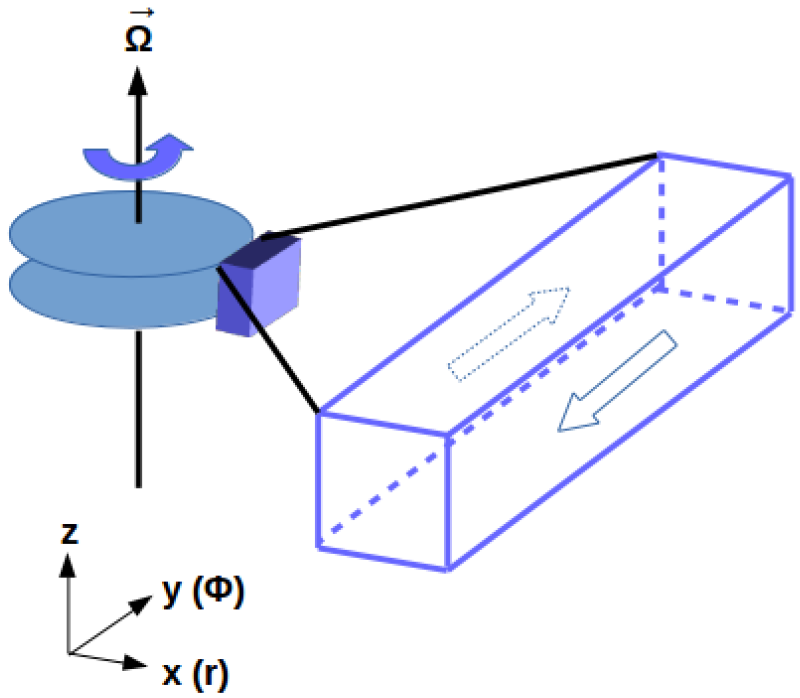
\includegraphics[width=0.9\linewidth]{./contents/shearing_box_TMD.png}
  \caption{shearing--boxの模式図. 円盤の一部を曲率が無視できるくらい小さな箱として切り出し, その中で流体シミュレーションを行う. \url{https://www.astr.tohoku.ac.jp/~tomida/athena/modules.html}}\label{fig:TMDbox}
 \end{figure}
%========================================================================%
\section{Results}
図\ref{fig:colourbar}に, 各時刻$t$の高さ$z/H$におけるMaxwell応力テンソルの$R\phi$成分$T^{\mathrm{Max}}_{R\phi}$を示した. 上下のパネルはそれぞれ(1)オーム散逸のみ (2)オーム散逸と両極性拡散 の結果に対応する. %シミュレーションの結果は\( -8 < z/H < 8 \)の領域で示されているが, 以降は\( 0 < z/H < 8 \)の領域のみ
\par
オーム散逸のみ(パネル上部)の場合, \( z/H > 2 \)の領域ではギザギザした形状が確認できる. これは, \( z/H > 2 \)の領域ではオーム散逸が効かず, MRIが成長したことにより生じたものと解釈できる. \( 0 < z/H < 2 \)にて比較的強い応力が見られるのは, \( z/H > 2 \)で生じた乱流が円盤中央へ伝播したからと考えられる. 
\par
両極性拡散も含めた(パネル下部)場合,  \( z/H > 2 \)の領域では, ギザギザした形状分布ではなく, 層状分布が現れた. これは両極性拡散が\( 2 < z/H < 4 \)の領域附近で効き, MRIが抑制されたからと考えられる. \figref{fig:Rphi_stress}より, \( z<4H \)における応力テンソルの$R\phi$成分$T_{R\phi}$を見積もると\( T_{R\phi} \approx \num{3e-4}\rho_0 c_s^2 \)となった(\( \rho_0 = \SI{13.1e-8}{g.cm^{-3}} \)). 
%========================================================================%
\begin{figure}\label{fig:colourbar}
  \centering
  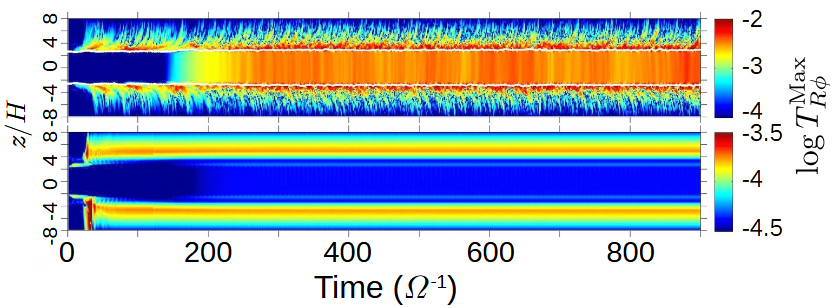
\includegraphics[width=1\linewidth]{./contents/colorbarMRI.png}
  \caption{Maxwell応力テンソル$T^{\mathrm{Max}}_{R\phi}$の時間--空間分布. 上下のパネルはそれぞれ(1)オーム散逸のみ (2)オーム散逸と両極性拡散 の結果を示している. (1)オーム散逸のみの場合, \( z>4H \)でMRIが発達している; (2)両極性拡散も含めると, \( z>4H \)で両極性拡散が効き, MRIが抑制される.}
\end{figure}
\begin{figure}\label{fig:Rphi_stress}
  \centering
  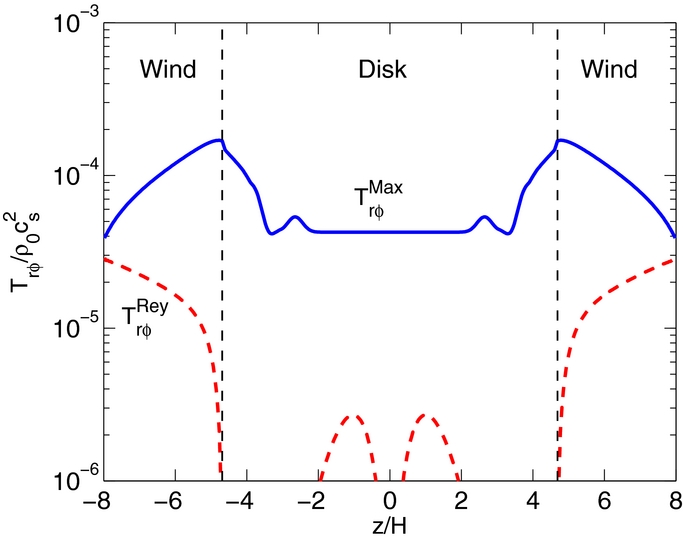
\includegraphics[width=1\linewidth]{./contents/figure8.jpg}
  \caption{応力テンソルの$R\phi$成分$T_{R\phi}$の分布. オーム散逸が効いている領域\( z<4H \)では, $T_{R\phi}$はほとんど一定の値\( T_{R\phi} \approx \num{3e-4}\rho_0 c_s^2 \)をとっている(\( \rho_0 = \SI{13.1e-8}{g.cm^{-3}} \)).}
\end{figure}
% \begin{figure}
%   \centering
%   \includegraphics[width=0.8\linewidth]{../figure6.jpg}
%   \caption{}
% \end{figure}
%========================================================================%
\section{Discussion}
式\eqref{eq:alphaparametor}, \eqref{eq:accretionrate}から, 両極性拡散を含むシミュレーションで得た応力テンソルの値を用いて降着率$\dot{M}$を計算すると\( \dot{M} \approx \num{2e-9} M_{\odot}\, \si{yr^{-1}} \)となった. これは観測値の誤差範囲内であるが, 中央値よりはやや小さい値となっている. 
\par
Bai \& Stone 2013では, MRIに代わる角運動量輸送として磁気遠心力風に着目した. 実際, 今回のシミュレーションでは\figref{fig:v_distribution}の速度分布を得ており, 円盤上部で磁気遠心力風が吹いていると考えられる. 
\par
ここで磁気遠心力風の簡単な説明を行う. 原始星の回転により強化された磁場は\figref{fig:magnetocentrifugal_wind}のような磁力線を描く. 磁気圧を受けたプラズマは磁力線にそって円盤上方へ飛んでいき, 磁気遠心力風を構成する. 
\par
\begin{figure}\label{fig:v_distribution}
  \centering
  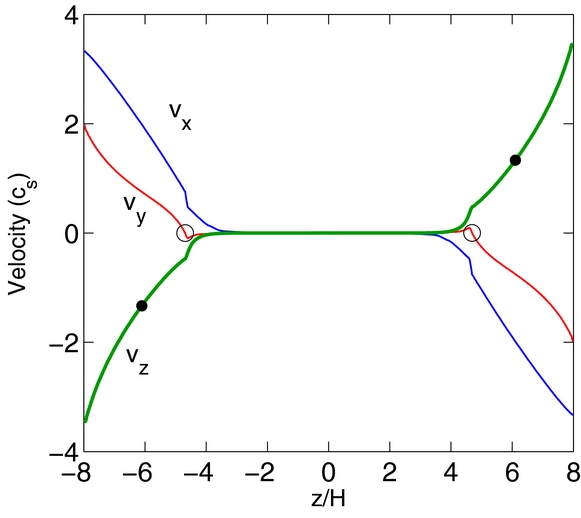
\includegraphics[width=1\linewidth]{./contents/v_distribution.png}
  \caption{オーム散逸と両極性拡散を考慮したシミュレーションにおけるガスの速度分布. 分布は準定常状態(\(\Omega t > 300\))における値である. 円盤の上部(\( z>4H \))で$v_z$が増加している.}
\end{figure}
\par
磁気遠心力風を考慮して円盤の降着率を再計算する. 式\eqref{eq:accretionrate}の右辺へ磁気遠心力風の寄与
\begin{equation}
  \frac{4\pi}{\Omega} R T_{\phi z}|_{-z_b}^{z_b} = \frac{8\pi}{\Omega} RT_{\phi z}|_{z_b}
\end{equation}
を加えて計算すると\( \dot{M} \approx \num{4.3e-8} M_{\odot} \si{yr^{-1}} \)を得た. これは磁気遠心力風を考慮していない場合に比べて, より観測値を再現している. 
\begin{figure}\label{fig:magnetocentrifugal_wind}
  \centering
  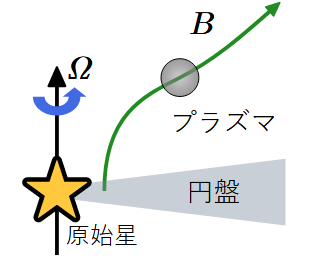
\includegraphics[width=1\linewidth]{./contents/magnetocentrifugal_wind.png}
  \caption{磁気遠心力風の模式図. 原始星の回転により強化された磁場がプラズマを磁力線方向へ吹き飛ばす.}
\end{figure}
%=================================================================================================%
\section{Conclusion}
 今回紹介したBai \& Stone 2013では, 原始惑星系円盤における降着メカニズムを調べるため, オーム散逸と両極性拡散の両方を考慮した3次元MHDシミュレーションを行った. 両極性拡散はMRIを強く抑制するため, MRIのみで円盤の降着率を説明するのは十分でないことが分かった. しかし, 円盤上部で発生している磁気遠心力風も考慮して降着率を計算すると, 観測値により近い値を得ることができた. 
%=================================================================================================%
\begin{thebibliography}{9}
  \bibitem{baiWinddrivenAccretionProtoplanetary2013a}
  Bai and Stone,
  ApJ, 769, 76 (2013)
  \bibitem{gullbringDiskAccretionRates1998}
  Gullbring et al.
  ApJ, 492, 323(1998)
  \bibitem{shakuraBlackHolesBinary1973}
  Shakura and Sunyaev,
  A\&A, 24, 337(1973)
  \bibitem{baiRoleTinyGrains2011}
  Bai
  ApJ, 739, 51(2011)
  \bibitem{balbusPowerfulLocalShear1991}
  Balbus and Hawley,
  ApJ, 376, 214(1991)
  \bibitem{hawleyLocalThreedimensionalMagnetohydrodynamic1995}
  Hawley et al.
  ApJ, 440, 742(1995)
\end{thebibliography}
\end{document}